\documentclass[12pt]{report}
\usepackage[a4paper]{geometry}
\usepackage[utf8]{inputenc}
\usepackage[english,portuguese]{babel}
\usepackage[myheadings]{fullpage}
\usepackage[T1]{fontenc}
\usepackage{fancyhdr}
\usepackage{graphicx, setspace}
\usepackage{sectsty}
\usepackage{url}
\usepackage{pdfpages}
\usepackage{subcaption}
\usepackage{amsmath}
\usepackage{multirow}
\usepackage{tikz}
\usepackage{minted}
\usepackage{hyperref}
\usepackage{amsfonts}
\usepackage{bbm, dsfont}
\usepackage{tikz}
%\usetikzlibrary{positioning}
\usetikzlibrary{shapes,positioning,calc,quotes}
\tikzstyle{subrotina} = [rectangle, draw,text centered, minimum width=5em, inner sep=5pt]
\tikzstyle{funcao} = [rounded rectangle, draw, text centered, minimum width=7em, inner sep=5pt]
\tikzstyle{random} = [rectangle, text centered, inner sep=5pt, minimum width=5em]
\tikzstyle{loop} = [rectangle, draw, align=left]
\tikzstyle{fluxo} = [draw, thick, -latex]
\tikzstyle{meiofluxo} = [draw, -]
\tikzstyle{chamada} = [draw, dashed, <->]


%%------ 
%% Comandos gerais
%% Observação: o arquivo "comandos.tex" tem que estar presente.
%%------
%%%%%%%%%%%%%%%%%%%%%%%%%%%%%%%%%%%%%%%%%%%%%%%%%%%%%%%%%%%%%%%%%%%%%
% In English:
%    This is a list of commands specification for FAPESP reports.
%
% In Portuguese:
%    Esta é uma lista de especificação de comandos para relatórios
% da Fundação de Amparo à pesquisa do Estado de São Paulo (FAPESP).
%
% Author/Autor: André Leon Sampaio Gradvohl, Dr.
% Email:        andre.gradvohl@gmail.com
% Lattes CV:    http://lattes.cnpq.br/9343261628675642
% 
% Last update/Última versão: 11/Sep/2016
%%%%%%%%%%%%%%%%%%%%%%%%%%%%%%%%%%%%%%%%%%%%%%%%%%%%%%%%%%%%%%%%%%%%%%

\def\checkmark{\tikz\fill[scale=0.4](0,.35) -- (.25,0) -- (1,.7) -- (.25,.15) -- cycle;}

\DeclareMathOperator{\diag}{diag}
\DeclareMathOperator{\ai}{Ai}
\DeclareMathOperator{\re}{Re}
\DeclareMathOperator{\im}{Im}
\DeclareMathOperator{\ee}{\rm e}
\DeclareMathOperator{\supp}{supp}
\renewcommand{\Re}{\mathop{\rm Re}}
\newcommand{\res}{\mathop{\rm Res}}
\renewcommand{\Im}{\mathop{\rm Im}}
\newcommand{\N}{\mathbb{N}}
\newcommand{\C}{\mathbb{C}}
\DeclareMathOperator{\Tr}{Tr}
\newcommand{\R}{\mathbb{R}}
\newcommand{\Z}{\mathbb{Z}}
\newcommand{\D}{\mathbb{D}}
\newcommand{\Q}{\mathbb{Q}}
\newcommand{\boh}{\mathit{o}}
\newcommand{\Boh}{\mathcal{O}}
\newcommand{\bbp}{\bm K_{\mathrm{BBP}}}
\newcommand{\ii}{\mathrm{i}}
\newcommand{\dd}{\mathrm{d}}
\newcommand*{\deff}{\mathrel{\vcenter{\baselineskip0.5ex \lineskiplimit0pt
			\hbox{\scriptsize.}\hbox{\scriptsize.}}}%
	=}
\newcommand*{\revdeff}{=\mathrel{\vcenter{\baselineskip0.5ex \lineskiplimit0pt
			\hbox{\scriptsize.}\hbox{\scriptsize.}}}%
}

\newcommand{\HRule}[1]{\rule{\linewidth}{#1}}
\setcounter{tocdepth}{3}
\setcounter{secnumdepth}{3}

\newcommand{\titulo}[1]{\def\meuTitulo{#1}}
\newcommand{\tituloIngles}[1]{\def\meuTituloIngles{#1}}
\newcommand{\numProjeto}[1]{\def\numFAP{#1}}
\newcommand{\tipoRelatorio}[1]{\def\tipoRelat{#1 }} %o espaço depois do #1 é importante
\newcommand{\modalidadeProjeto}[1]{\def\modProjeto{#1}} 
\newcommand{\agFomento}[2]{\def\agFom{#1} \def\siglaAgFom{#2}} %extenso Sigla
\newcommand{\autor}[1]{\def\nomeAutor{#1}}
\newcommand{\cidade}[1]{\def\nomeCidade{#1}}
\newcommand{\universidade}[1]{\def\nomeUniversidade{#1}}
\newcommand{\faculdade}[1]{\def\nomeFaculdade{#1}}
\newcommand{\periodoVigencia}[1]{\def\periodVig{#1}}
\newcommand{\periodoRelatorio}[1]{\def\periodRelat{#1}}

\author{}
\date{}

%Definição de membros da equipe de pesquisas
\newcommand{\membroA}[1]{\def\nomeMembroA{#1}}
\newcommand{\membroB}[1]{\def\nomeMembroB{#1}}
\newcommand{\membroC}[1]{\def\nomeMembroC{#1}}
\newcommand{\membroD}[1]{\def\nomeMembroD{#1}}
\newcommand{\membroE}[1]{\def\nomeMembroE{#1}}
\newcommand{\membroF}[1]{\def\nomeMembroF{#1}}

\newcommand{\Figure}[1]{Figura~\ref{fig:#1}}
\newcommand{\Table}[1] {Tabela~\ref{#1}}
\newcommand{\Equation}[1] {Equa\c{c}\~ao~\ref{#1}}
\newcommand{\addFigure}[3] { %Parametros scale, fig_name, caption 
    \begin{figure}[!hbt]
      \centering
      \includegraphics[scale=#1]{figures/}
      \caption{#3}\label{fig:#2}
    \end{figure}
}

\newcommand{\geraTitulo}{
\clearpage
\begin{titlepage}
  \begin{center}
      \vspace*{-3cm}
       { \setstretch{.5} 
         \textsc{\nomeUniversidade} \\
         \HRule{.2pt}\\
         \textsc{\nomeFaculdade}
       }

       \vspace{5.5cm}

       \Large \textbf{\textsc{\meuTitulo}}
 	  \HRule{1.5pt} \\ [0.5cm]
       \linespread{1}
       \large Relatório Científico 
       \ifdefined\tipoRelat
            \tipoRelat
       \fi
       do projeto 
       \ifdefined\modProjeto
           na modalidade \modProjeto,
       \fi
       fomentado pela \agFom. \\ 
   	   \HRule{1.5pt} \\ [0.5cm]

       \ifdefined\numFAP
          Projeto \siglaAgFom~\texttt{\#\numFAP}
          \\ [0.5cm]
       \fi
        Pesquisador Responsável: \nomeAutor
        
        \hspace{2cm}
        
        
\includegraphics[scale=0.7]{Assets/CuteCircleWhite}
       
        \vfill
       
        {\normalsize  \nomeCidade, \today}
 \end{center}
 \end{titlepage}
}

\usepackage{titlesec}
\titleformat{\chapter}{\normalfont\LARGE\bfseries}{\thechapter}{1em}{}
\titlespacing*{\chapter}{0pt}{3.5ex plus 1ex minus .2ex}{2.3ex plus .2ex}

%----------------------------------------------------------------------
% Cabeçalho e rodapé
%----------------------------------------------------------------------
\pagestyle{fancy}
\fancyhf{} % Limpa todos os campos de header and footer fields
\renewcommand{\headrulewidth}{0pt}
\fancyfoot[R]{\thepage}

\addto\captionsportuguese{\renewcommand{\contentsname}{Sumário}}
\addto\captionsportuguese{\renewcommand{\bibname}{Referências Bibliográficas}}

%------
% Resumo e Abstract
%------
\newcommand{\Resumo}[1]{
   \begin{otherlanguage}{portuguese}
       \addcontentsline{toc}{chapter}{Resumo}
       \begin{abstract} \thispagestyle{plain} \setcounter{page}{2}
          #1
        \end{abstract}
   \end{otherlanguage} 
} %end \Resumo

\newcommand{\Abstract}[1]{
   \begin{otherlanguage}{english}
      \addcontentsline{toc}{chapter}{Abstract}
      \begin{abstract} \thispagestyle{plain} \setcounter{page}{3}
       #1
      \end{abstract}    
    \end{otherlanguage} 
} %end \abstract

%------
% Folha de rosto
%------
\newcommand{\folhaDeRosto}{
   \chapter*{Informações Gerais do Projeto}
   \addcontentsline{toc}{chapter}{Informações Gerais do Projeto}
   \begin{itemize}
      \item Título do projeto: 
            \begin{itemize}\item[] \textbf{\meuTitulo} \end{itemize}
      \item Nome do pesquisador responsável: 
            \begin{itemize}\item[]\textbf{\nomeAutor}\end{itemize}
      \item Instituição sede do projeto: 
            \begin{itemize}
               \item[]\textbf{\nomeFaculdade \ da \nomeUniversidade} 
            \end{itemize}
      \item Equipe de pesquisa:
            \begin{itemize}
               \ifdefined\nomeMembroA
                 \item[]\textbf{\nomeMembroA}
               \else 
                 \item[]\textbf{\nomeAutor}
               \fi
               \ifx\nomeMembroB\undefined\else \item[]\textbf{\nomeMembroB}\fi
               \ifx\nomeMembroC\undefined\else \item[]\textbf{\nomeMembroC}\fi
               \ifx\nomeMembroD\undefined\else \item[]\textbf{\nomeMembroD}\fi
               \ifx\nomeMembroE\undefined\else \item[]\textbf{\nomeMembroE}\fi
               \ifx\nomeMembroF\undefined\else \item[]\textbf{\nomeMembroF}\fi
             \end{itemize}
       
          \ifdefined \numFAP
             \item Número do projeto de pesquisa:
             \begin{itemize}
                 \item[]\textbf{\numFAP} 
             \end{itemize}
          \fi  
       \item Período de vigência:
            \begin{itemize}
               \item[]\textbf{\periodRelat} 
            \end{itemize}
       \item Período coberto por este relatório científico:
            \begin{itemize}
               \item[]\textbf{\periodVig} 
            \end{itemize}
   \end{itemize}
   \clearpage
}


\newcommand\underrel[2]{\mathrel{\mathop{#2}\limits_{#1}}}

\newcommand{\matriz}[1]{\hat#1}

\newcommand{\many}[2]{$#1_1, #1_2, \dots, #1_#2$}

\newcommand{\cmany}[3]{$#1_1 #3 #1_2 #3 \dots #3 #1_#2$}

\newcommand{\mmany}[2]{ #1_1, #1_2, \dots, #1_#2 }

\newcommand{\mcmany}[3]{#1_1 #3 #1_2 #3 \dots #3 #1_#2}

\newcommand{\set}[1]{\{#1\}}

\newcommand{\cjgt}[1]{\overline{#1}}
\DeclareMathOperator{\sign}{sign}
\DeclareMathOperator{\Df}{D}
\DeclareMathOperator{\Ee}{E}
\DeclareMathOperator{\h}{h_1}
\DeclareMathOperator{\f}{f}
\DeclareMathOperator{\U}{U}
\DeclareMathOperator{\W}{W}
\DeclareMathOperator{\K}{K}
\DeclareMathOperator{\Hf}{\mathcal{H}}
\DeclareMathOperator{\Qf}{Q}
\DeclareMathOperator{\Gl}{\mathcal{L}}
\DeclareMathOperator{\g}{g}
\DeclareMathOperator{\V}{V}
\newcommand{\iu}{\mathrm{i}\mkern1mu}
\renewcommand{\Im}{\mathop{\textrm Im}}
\newcommand{\J}{J} %Jacobiano
\newcommand{\Id}{\mathbb{1}}
\newcommand{\p}{\mathcal{P}} %medida
\newcommand{\Se}{\mathbb{S}}
\newcommand{\He}{\mathbb{H}}
 \newcommand{\E}{\mathbb{E}}

% MATH DECLARATIONS
\newtheorem{lemma}{Lema}[section]
\newtheorem{thm}[lemma]{Teorema}
\newtheorem{claim}[lemma]{Afirmação}
\newtheorem{cor}[lemma]{Corolário}
\newtheorem{definition}[lemma]{Definição}
\newtheorem{conjecture}[lemma]{Conjectura}
\newtheorem{prop}[lemma]{Proposição}
\newtheorem{assumption}[lemma]{Assumpção}
\numberwithin{equation}{section} %numeracao dentro de secoes

% PROOF ENV
\makeatletter
\newenvironment{proof}[1][Demonstração]{\par
	\pushQED{\qed}%
	\normalfont \topsep6\p@\@plus6\p@\relax
	\trivlist
	\item\relax
	{\itshape
		#1\@addpunct{.}}\hspace\labelsep\ignorespaces
}{%
	\popQED\endtrivlist\@endpefalse
}
\makeatother
%%-----
%% Página de título
%% Observação: As definições que aparecem a seguir comporão a
%%             página de título e a folha de rosto.
%%-----
%% Define o nome da universidade onde o projeto foi desenvolvido.
\universidade{Universidade de São Paulo}
%
%% Define o nome da faculdade onde o projeto foi desenvolvido.
\faculdade{Instituto de Ciências Matemáticas e de Computação (ICMC)}
%
%% Define o título do projeto.
\titulo{Matrizes aleatórias e simulação de gases de Coulomb}
%
%% Define a agencia de Fomento e a abreviatura. O primeiro argumento é o 
%% nome por extenso e o segundo a abreviatura.
%% Ambos os argumentos são obrigatórios
\agFomento{Fundação de Amparo à Pesquisa do Estado de São Paulo}{FAPESP}
%
%% Define o tipo de relatório. Pode ser Anual ou Final.
%% Não é obrigatório definir o tipo de relatório.
\tipoRelatorio{Final}
%
%% Define a modalidade de Projeto. Pode ser temático, regular, etc.
\modalidadeProjeto{Iniciação Científica}
%
%% Define o número do projeto.
%% Não é obrigatório definir o número do projeto.
\numProjeto{2023/02674-0} 
%
%% Define o autor do relatório.
\autor{Guilherme L. F. Silva}
%
%% Define a equipe do projeto (incluindo o pesquisador responsável no comando \membroA{}
\membroA{Guilherme L. F. Silva}
%% Inclua os demais membros do grupo (máximo +5)
\membroB{João Victor Alcantara Pimenta}
%\membroC{Francisco}
%\membroD{Joao}
%\membroE{Antonio}
%\membroF{José}
%
%% Define o período da vigência do Projeto.
\periodoRelatorio{01/06/2023 a 31/05/2024}
%
%% Define o período coberto pelo relatório.
\periodoVigencia{01/06/2023 a 31/05/2024}
%
%% Define a cidade onde o projeto foi desenvolvido.
\cidade{São Carlos}

%%-----
%% Página de título
%% Observação: Os comandos a seguir não devem ser mudados, 
%%             exceto caso necessário.
%%-----
\begin{document}
%
%% Define a numeração em romanos.
\pagenumbering{roman}
%
%% Gera a folha de título.
\geraTitulo
%
%% Gera a folha de rosto.
\folhaDeRosto
%
%% Escreva aqui o resumo em português.
\Resumo{
  O estudo de Matrizes Aleatórias demonstra aplicabilidade em uma gama diversa de áreas, com
  destaque no estudo de mecânica estatística, principalmente na simulação de gases. Estudando a
  densidade espectral de sistemas de matrizes Gaussianas pode-se desenvolver uma analogia que
  possibilita a simulação de sistemas de gases diversos, como o de Coulomb. Algumas dificuldades
  surgem na implementação de simulações baseadas nesta teoria, principalmente em escalabilidade do sistema e no tratamento de possíveis singularidades. Para resolver estes problemas,
  abordou-se na simulação na literatura, dentre outros, o Algoritmo Híbrido de Monte Carlo, de
  ótimo comportamento numérico. Nosso objetivo é explorar este assunto, as simulações de gases
  e o algoritmo citado acima além de expandir os potenciais em que foi-se bem documentado o
  comportamento destas simulações.
  }
%
%% Escreva aqui o resumo em inglês.
% \Abstract{
%	The study of Random Matrices demonstrates applicability in a diverse range of areas, empha-
%	sizing the study of statistical mechanics, mainly in the simulation of gases. By studying the
%	spectral density of Gaussian matrix systems, one can develop the simulation of Coulomb gas
%	systems in analogy. Some difficulties arise in implementing simulations based on this theory,
%	mainly in system scalability and the treatment of possible singularities. To solve these pro-
%	blems, the literature has simulated these gases, with excellent numerical behavior, using the
%	Monte Carlo Hybrid Algorithm. We wish to explore this problem, the simulations, and the
%	proposed algorithm along with extending the potentials to wich it has been tested.
%}
%
%% Adicionará o sumário.
%% Mantenha o \thispagestyle{empty} e \clearpage
\thispagestyle{empty}
\clearpage
%
%% Define a numeração em arábicos.
\pagenumbering{arabic}

%%-----
%% Formatação do título da seção
%%-----
\sectionfont{\scshape}

%%-----
%% Corpo do texto
%%-----

\chapter{Atividades Desenvolvidas}
\label{section:atividadesdesenvolvidas}

A execução do projeto foi dividida nas seguintes etapas:

\begin{enumerate}
	\item \textbf{Revisão da Literatura em RMT, e estudo de teoria básica do GUE}, é necessário fazer vasta revisão de literatura no tema para que o aluno tenha domínio das ferramentas e métodos utilizados para o tratamento de matrizes aleatórias e suas implicações em mecânica estatística. Para isso, durante esse período será realizado o estudo da bibliografia adequada;
	
	\item \textbf{Estudo dos métodos de Simulação}, como mencionado, uma das aplicações importantes da teoria de matrizes aleatórias reside em sua conexão com gases de Coulomb. Em 2018 publicou-se o artigo \cite{Chafa2018}, base para o estudo do método de simulação implementado;
	
	\item \textbf{Implementação dos algoritmos}, implementa-se os métodos descritos no artigo e tenta-se estender seu uso em condições diferentes das utilizadas no artigo, como por exemplo em outros potenciais;
	
	\item \textbf{Redação dos Relatórios Científicos}, quando serão escritos os relatórios exigidos pelas normas da \textit{FAPESP}.
	
\end{enumerate}

\section{Cronograma}

Com base nas tarefas enumeradas na Seção \ref{section:atividadesdesenvolvidas}, é mostrado na Tabela \ref{tab:cronograma1ano} o cronograma atual de desenvolvimento do projeto. Foi possível realizar todo o planejamento feito inicialmente.

%\begin{table}[ht]
%\centering
%\begin{tabular}{|c|c|c|c|c|c|c|c|c|c|c|c|c|}
%\hline
%\multirow{2}{*}{{\bf Fases}} & \multicolumn{6}{c|}{{\bf Meses}}
%\\ \cline{2-7}
%    & 1 & 2 & 3 & 4 & 5 & 6
%\\ \hline
%    {\bf 1. Revisão Literatura RMT} & x & x & x & & &  
%\\ \hline
%    {\bf 2. Métodos de Simulação} &  &  & x & x & &
%\\ \hline
%    {\bf 3. Implementação algoritmos} & & & & x & x & 
%\\ \hline
%    {\bf 4. Redação Relatórios} & & & & & & x
%\\ \hline
%\end{tabular}
%\caption{Cronograma das atividades.}
%\label{tab:cronograma6meses}
%\end{table}

\begin{table}[ht]
	\centering
	\begin{tabular}{|c|c|c|c|c|c|c|c|c|c|c|c|c|}
		\hline
		\multirow{2}{*}{{\bf Fases}} & \multicolumn{12}{c|}{{\bf Meses}}
		\\ \cline{2-13}
		& 1 & 2 & 3 & 4 & 5 & 6 & 7 & 8 & 9 & 10 & 11 & 12
		\\ \hline
		{\bf 1. Revisão Literatura RMT} & \checkmark & \checkmark & \checkmark & \checkmark & \checkmark & & & & & & &
		\\ \hline
		{\bf 2. Métodos de Simulação} &  &  &  & \checkmark & \checkmark & \checkmark & \checkmark & \checkmark & & & &
		\\ \hline
		{\bf 3. Implementação algoritmos} & & & & & \checkmark & \checkmark & \checkmark & \checkmark & \checkmark & \checkmark & \checkmark &
		\\ \hline
		{\bf 4. Redação Relatórios} & & & & \checkmark & \checkmark & & & & & & \checkmark & \checkmark 
		\\ \hline
	\end{tabular}
	\caption{Cronograma das atividades.}
	\label{tab:cronograma1ano}
\end{table}

\chapter{Realizações do período}\label{chp:realizacoes}

\section{Graduação}

Durante o período referente à pesquisa o aluno realizou as seguintes matérias e respectivos desempenhos:
\hspace{1cm}

\begin{center}
	\begin{tabular}{|c|c|c|c|}
		\hline
		Disciplina & Sigla & Nota & Semestre \\
		\hline
		Mecânica Estatística Avançada & 7600041 & 10.0 & 1 - 2023 \\
		\hline
		Introdução aos Sistemas de Computação & 7600056 & 9.2 & 1 - 2023 \\
		\hline
		Física Estatística Computacional & 7600073 & 9.7 & 1 - 2023 \\
		\hline
		Teoria Espectral de Matrizes & SME0243 & 10.0 & 1 - 2023 \\
		\hline
		Mecânica Quântica & 7600022 & 9.3 & 2 - 2023 \\
		\hline
		Física Matemática Avançada & 7600034 & 10.0 & 2 - 2023 \\
		\hline
		Noções Básicas de Fabricação Mecânica & 7600134 & 10.0 & 2 - 2023 \\
		\hline
		Espaços Métricos & SMA0343 & 9.0 & 2 - 2023 \\
		\hline
		Laboratório Avançado de Física 1& 7600024 & - & 1 - 2024 \\
		\hline
		Álgebra 1 & SMA0305 & - & 1 - 2024 \\
		\hline
		Trabalho de Conclusão de Curso & 7600039 & - & 1 - 2024 \\
		\hline
	\end{tabular}
\end{center}

\section{Participação em eventos científicos}\label{chp:particEvento}

Durante o período de 13 de Janeiro à 24 de Fevereiro o bolsista participou do evento 'Jornadas de Pesquisa em Matemática' realizado pelo Instituto de Ciências Matemáticas e de Computação (ICMC - USP). Durante este evento foi realizado pesquisa original em simulações de caminhos aleatórios, que rendeu o relatório de nome 'Baralhos e passeios aleatórios', submetido para a FAPESP e disponível em anexo.

O bolsista também apresentou em dois eventos no período da pesquisa. O Colóquio Brasileiro de Matemática (CBM) e a Semana Integrada da Física de São Carlos (SIFSC). Apenas para o primeiro, realizado no Rio de Janeiro, foi necessário o uso da reserva técnica. Por isso, segue o pôster apresentado na página que se segue. O trabalho é complementar aos estudos assintóticos e de probabilidade realizados nos meses cobertos por este relatório.

\hspace{1cm}

\begin{tabular}{|c|c|c|c|c|c|}
	\hline
	Evento &  Sede & Data & Modalidade & Apresentação & Reserva Técnica \\
	\hline
	CBM & IMPA & 24-28/07/23 & Presencial & Pôster - Oral & Sim \\
	\hline
	SIFSC & IFSC-USP & 21-25/08/23 & Presencial & Pôster - Oral & Não \\
	\hline
	Jornadas & ICMC-USP & 13/01-24/02/23 & Presencial & Oral & Não \\
	\hline
\end{tabular}

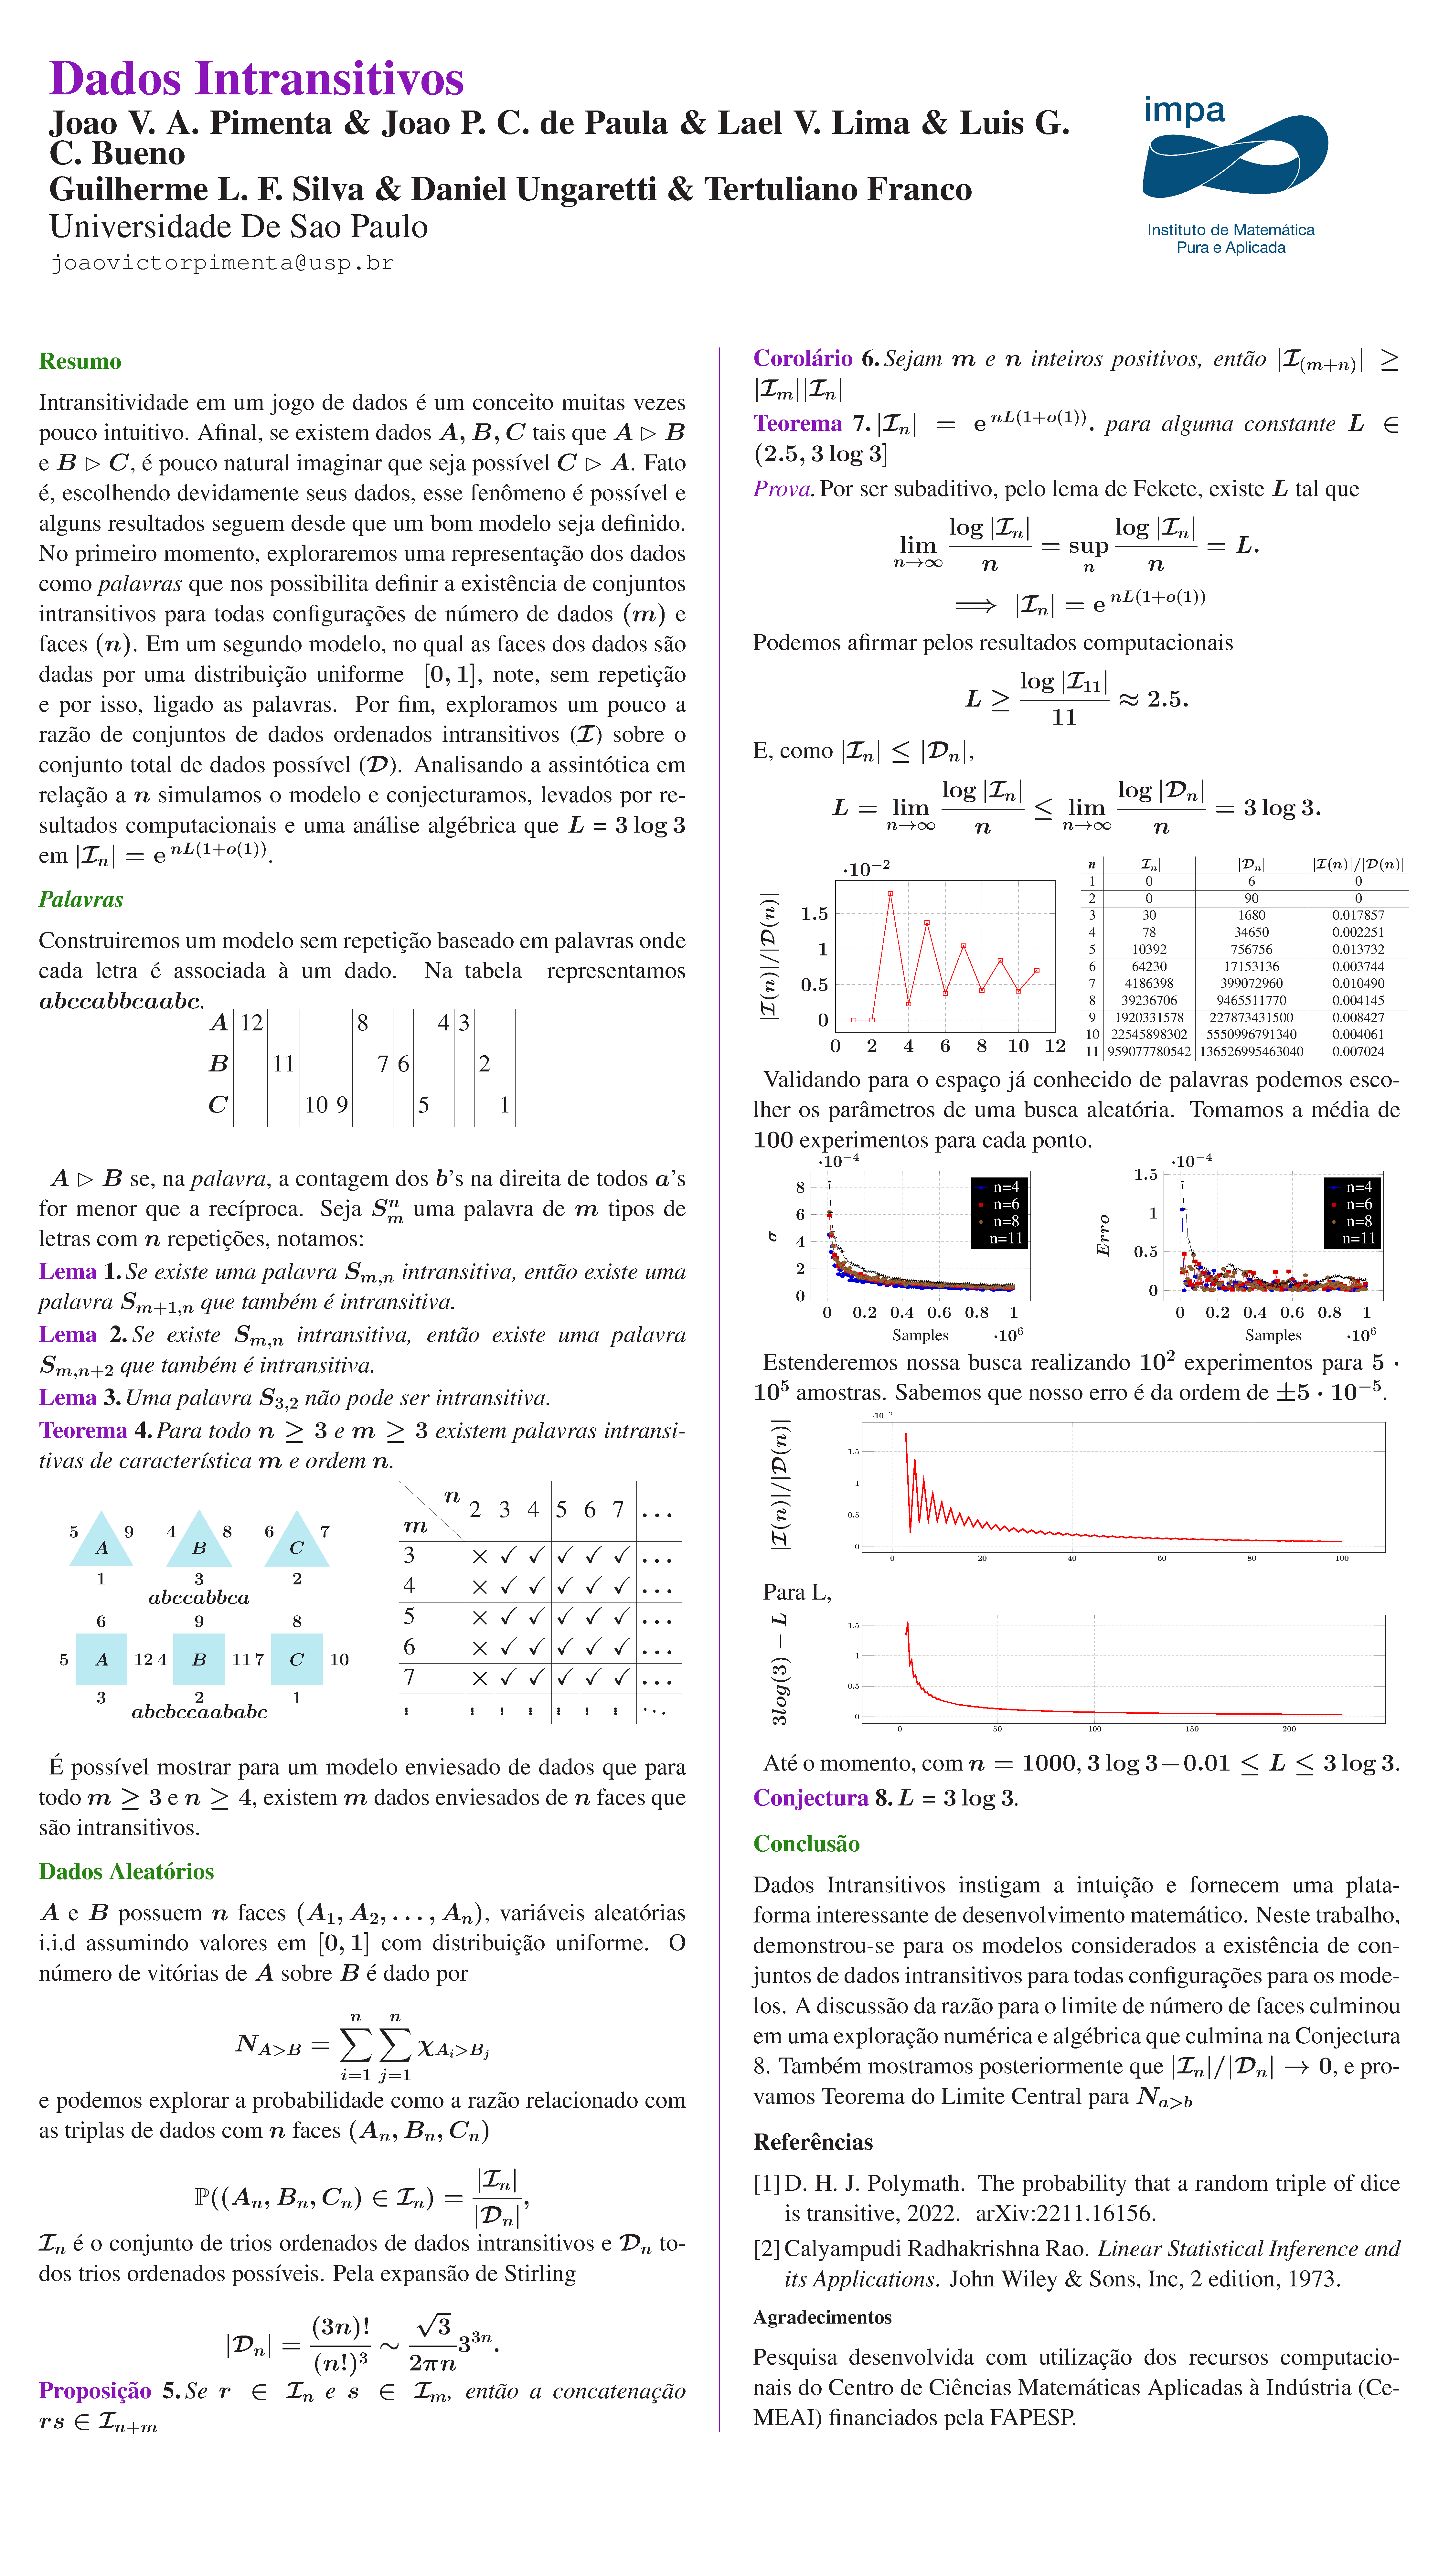
\includepdf[pages={1}]{Assets/posterwhite.pdf}

\section{Outros trabalhos Preparados ou Submetidos}

Durante o período da bolsa foi também finalizado o trabalho intitulado ’A Central Li-
mit Theorem for intransitive dice’ co-autorado por mim. O arquivo se encontra disponível
na plataforma Arxiv em \url{https://arxiv.org/abs/2310.17083}. Por fim, realizou-se o desenvolvimento do Trabalho de Conclusão de Curso referente à graduação em andamento. A ser defendido, disponível em anexo.

\section{Pesquisa}
\label{Pesquisa}

Os resultados e texto científico abaixo foram desenvolvidos conjuntamente com o trabalho de conclusão de curso realizado no mesmo período, tomando como base seu conteúdo. Apresento breve noção do trabalho e alguns resultados e possibilidades para desenvolvimento e uso destes. Todos os produtos, programas e textos, podem ser acessados em \url{https://github.com/Joao-vap/RMT-TEX} e \url{https://github.com/Joao-vap/RMT-Code}.

\subsection{Matrizes Aleatórias}

De acordo com a mecânica quântica, níveis de energia de uma sistema são descritos pelos autovalores de seu operador hermitiano associado, o hamiltoniano $\Hf$. Em situações mais complexas, $\Hf$ não é completamente descrito pela teoria ou é complicado. Por isto, somado à necessidade do cálculo explícito de grandezas, considera-se usualmente truncamentos do espaço de Hilbert onde opera $\Hf$, representado agora por matriz de dimensão finita. Caracterizar o sistema físico é resolver o problema de autovalores $\Hf \Psi_i = E_i \Psi_i$.

Wigner, em seu estudo de núcleos atômicos, sugere uma solução alternativa, uma mecânica estatística para o problema de autovalores. Tal teoria descreveria, estocasticamente, o perfil da estrutura energética nucleica ao invés de detalhar seus níveis. Buscava-se, em algum sentido, uma universalidade, uma resposta que fosse, dada complexidade o suficiente, independente de $\Hf$. A teoria foi prontamente seguida por, dentre outros, Porter e Rosenzweig \cite{PoterRosen}, que procederam a validar com dados experimentais as ideias postuladas e por Gaudin, Mehta \cite{MehtaGaudin}, e Dyson \cite{Dyson}, que avançaram na descrição, dentre outros, dos importantes ensembles gaussianos. Esse desenvolvimento é o início da chamada Teoria de Matrizes Aleatórias (RMT, \textit{Random Matrix Theory}) e hoje desempenha importante papel na descrição estatística de sistemas com alta complexidade representados com matrizes de simetria induzida pela natureza do problema descrito.

Seja $\Se$ um conjunto tal como $\R, \C, \He $ (Reais, Complexos e Quaterniônicos). Considere uma matriz $\matriz{M} \in \mathcal{M}_{\Se}(N)$ espaço de matrizes $N \times N$, ou seja, de $N^2$ entradas, sejam elas reais, complexas ou quaterniônicas. Se tomamos o elemento de matriz $M_{i,j}$ $\forall i, j \in \Z$, com $1 \leq i, j \leq N$, como variável aleatória de distribuição arbitrária, podemos expressar a densidade de probabilidade conjunta (jpdf, \textit{joint probability density function}) como $$\p(\hat{M}) \dd M = \p(M_{1,1}, \dots, M_{N,N}) \prod_{i,j=1}^{N} \dd M_{i,j}.$$

Não lidaremos, contudo, com uma classe tão ampla de matrizes. Tomamos $\matriz{M}$ matriz ortogonal, unitária ou simplética, a depender de $\Se$, o que resulta em autovalores $\lambda \in \R$ sem degeneração. Isto pode ser motivado fisicamente sabendo que, para sistemas quânticos invariantes reversíveis, o Hamiltoniano é matriz real simétrica; na presença de campo magnético, o Hamiltoniano é matriz complexa hermitiana; na presença de acoplamento spin-órbita, o Hamiltoniano é simplético \cite[Capítulo~2]{RMT-firstcourse-Potters}. 

Considere a decomposição $\matriz{M} = \matriz{O} \matriz{D} \matriz{O}^{-1}$, com $\matriz{O} \in V_N(\Se^N)$ variedade de Stiefel e $\matriz{D} = \diag(\mmany{\lambda}{N})$. Se a transformação tem Jacobiano $\J(\matriz{M} \rightarrow \{ \vec{\lambda}, \matriz{O} \} )$, reescreve-se a jpdf em função dos autovalores e $\matriz{O}$ tal que:
\begin{equation}
	\p(\hat{M}) \dd M = \p \left( M_{1,1}(\vec{\lambda}, \matriz{O}), \cdots, M_{N,N}(\vec{\lambda}, \matriz{O}) | \J(\matriz{M} \rightarrow \{ \vec{\lambda}, \matriz{O} \} ) \right) \dd O \prod_{i=1}^{N} \lambda_i.
	\label{Equation: p(lambda, O)}
\end{equation}

Aqui, ressalta-se que estamos interessados em distribuições de autovalores. Para calcular $\p(\mmany{\lambda}{N})$ devemos integrar os termos à direita da equação \ref{Equation: p(lambda, O)} sobre o subespaço $V_N(\Se^N)$. Isso nem sempre é fácil ou possível. Para garantir integrabilidade, tomaremos \textit{ensembles} de matrizes aleatórias onde o jpdf de suas entradas pode ser escrito exclusivamente como função dos autovalores, ou seja $$\p(\mmany{\lambda}{N}, \matriz{O}) \equiv \p \left( M_{1,1}(\vec{\lambda}), \cdots, M_{N,N}(\vec{\lambda}) | \J(\matriz{M} \rightarrow \{ \vec{\lambda} \} ) \right).$$

Ensembles com esta propriedade são denominados invariantes (por rotação). Esta escolha implica que quaisquer duas matrizes $\matriz{M}, \matriz{M'}$ que satisfaçam a relação de equivalência $\matriz{M} = \matriz{U} \matriz{M'} \matriz{U}^{-1}$ tem mesma probabilidade. Nesta relação, $\matriz{U}$ é simétrica, hermitiana ou simplética respectivamente quando $\Se = \R,\C,\He $. Considere o teorema \cite[Capítulo~3]{AlanThesis}.
\begin{thm}
	Tome $\matriz{M} \in M_{\R}(N),  M_{\C}(N),  M_{\He}(N)$ simétrica, hermitiana ou autodual, respectivamente. Se  $\matriz{M}$ tem jpdf da forma $\phi(\matriz{M})$, invariante sobre transformações de similaridade ortogonal, a jpdf dos $N$ autovalores ordenados de $\matriz{M}$, $\mcmany{\lambda}{N}{\geq}$, é $$ C_{N}^{(\beta)} \phi(\matriz{D}) \prod_{i < j} (\lambda_i - \lambda_j)^{\beta}$$ onde $C_{N}^{\beta}$ é constante e $\beta = 1, 2, 4$ corresponde respectivamente à $\matriz{M} \in M_{\R}(N),  M_{\C}(N),  M_{\He}(N)$. 
	\label{Teorema: Invariante}
\end{thm}
Logo, desde que tomemos um ensemble invariante, podemos reescrever a distribuição em função dos autovalores pelo Teorema \ref{Teorema: Invariante}. Vale ainda observar que, pelo Lema de Weyl, uma jpdf invariante pode ser expressa totalmente por $\p(\matriz{M})= \phi \left(\Tr(F(M)) \right)$ com $F$ função polinomial. Ou seja, se unirmos os resultados do Teorema e Lema, podemos escrever
\begin{equation}
	\p_{ord}(\mmany{\lambda}{N}) = C_{N}^{\beta} \phi{\left( \sum_i^N F(\lambda_i) \right)} \prod_{i < j} (\lambda_i - \lambda_j)^{\beta}.
	\label{Equation: p-ord}
\end{equation}

Dentre os muitos ensembles em RMT, os Gaussianos são notórios. São eles o \textit{Gaussian Orthogonal Ensemble (GOE)} ($\beta=1$), \textit{Gaussian Unitary Ensemble (GUE)} ($\beta=2$) e \textit{Gaussian Sympletic Ensemble (GSE)} ($\beta=4$). Notemos primeiramente que o nome é relacionado à escolha de $\Se$. Mais explicitamente, o nome é dado em relação à se $\matriz{O}$, tal que $\matriz{M} = \matriz{O}\matriz{D}\matriz{O}^*$, é ortogonal, unitário ou simplético. É natural então pensar nos ensembles \textit{GOE}, \textit{GUE} e \textit{GSE} como matrizes $\matriz{M} \in \mathcal{M}_{\Se}(N)$ onde 
$$
\mathcal{M}_{\Se}(N) \ni M_{i,j} \sim
\begin{cases}
	\mathcal{N}_{\Se}(0,1/2) &  \ \text{para} \ i \neq j,\\
	\mathcal{N}_{\Se}(0,1) & \ \text{para} \ i = j.
\end{cases}
$$

Os três ensembles gaussianos compartilham de uma propriedade exclusiva - são os únicos ensembles com entradas independentes e, simultaneamente, jpdf rotacionalmente invariante. Podemos deduzir, para $\beta = 1,2,4$ que
\begin{equation}
	\p(\vec{\lambda}) = \frac{1}{Z_{N, \beta}} \ee^{-\beta_N \mathcal{H}_N(\vec{\lambda})},
	\label{Equation: medida Gaussian}
\end{equation}
onde $Z_{N, \beta}$ é função de partição canônica para autovalores desordenados\footnote{Usa-se do fator de contagem de Boltzmann para escrever $ Z_{N, \beta} = N! Z_{N, \beta}^{(ord)}$.}, normalizante da expressão \ref{Equation: medida Gaussian}. O fator $\beta_N = \beta N^2$ é pensado como a temperatura inversa. Definimos ainda o Hamiltoniano $$\mathcal{H}_N(\vec{\lambda}) = \frac{1}{N}\sum_{i = 1}^{N} \frac{\lambda_i^2}{2} + \frac{1}{N^2} \sum_{i < j} \log{\frac{1}{|\lambda_i - \lambda_j|}}$$ com  $\lambda_i \mapsto \lambda_i \sqrt{\beta N}$.

\subsection{Gases de Coulomb}

Para os ensembles que chamamos invariantes, a densidade de autovalores guarda uma importante analogia, a de Gases de Coulomb. Pensando os $N$ autovalores das matrizes como partículas de um gás com o devido núcleo de interação e potencial externo, podemos usar de noções físicas para intuir seu comportamento. Usando das estabelecidas leis termodinâmicas é possível ainda derivar, por exemplo, as densidades de autovalores no limite termodinâmico ($N \rightarrow \infty$). Generalizando o potencial aplicado podemos ainda recuperar um ensemble de matrizes que pode não estar diretamente disponível.

% Sabemos então, que a partir dessa função podemos retirar importantes propriedades estatísticas (macroscópicas) do sistema de autovalores dos ensembles Gaussianos.

O gás de coulomb $\p_N$ \cite{ChafaCoulombMeasure} é a medida de probabilidade de Boltzmann-Gibbs dada em $(R^d)^N$ por 
\begin{equation}
	\dd \p_N(\vec{x}) = \frac{e^{-\beta N^2 \Hf_N(\vec{x})}}{Z_{N,\beta}} \dd \vec{x},
	\label{Equação: Medida Gas de Coulomb}
\end{equation}
onde $$\Hf_N(\vec{x}) = \frac{1}{N} \sum_{i = 1}^{N} \V(x) + \frac{1}{2N^2} \sum_{i \neq j} \g(x_i - x_j)$$ é usualmente chamado hamiltoniano ou energia do sistema, $g$ é solução da equação de Poisson e $\V \colon \Se \mapsto \R$ potencial externo. A medida $\p_N$ modela um gás de partículas indistinguíveis com carga nas posições $\mmany{x}{N} \in \Se$ de dimensão $d$ em $\R^n$ \textit{ambient space}. As partículas estão sujeitas a um potencial externo $\V \colon \Se \mapsto \R$ e interagem por $\g \colon \Se \mapsto (-\infty, \infty]$. A temperatura inversa é $\beta N^2$. Assumiremos, para que valha a definição \ref{Equação: Medida Gas de Coulomb}, que $V, \ \g \ \text{e} \ \beta$ são tais que a constante de normalização (função partição) $Z_{N, \beta} < \infty \ \forall \ N$\footnote{Note que $\p_N$ é um modelo de interações estáticas e não há campos magnéticos considerados.}.

Se lembramos da expressão \ref{Equation: medida Gaussian}, perceberemos que, para o devido $\V(x)$, podemos tomar $d=1$ e $n = 2$ para recuperar a medida dos ensembles gaussianos 
\begin{equation}
	\p_N(\vec{x}) = \frac{e^{-\beta_N \Hf_N(\vec{x})}}{Z_{N,\beta}},
	\label{Equation: Medida Log V}
\end{equation}
\begin{equation}
	\Hf_N(\vec{x}) = \frac{1}{N} \sum_{i = 1}^{N} \V(x_i) + \frac{1}{N^2} \sum_{i < j} \log{\frac{1}{|x_i - x_j|}}.
\end{equation}
Estamos tratando de partículas no plano confinadas à uma reta. Para algum potencial arbitrário, além da devida escolha de $n$ e $d$, cairemos em outros ensembles de matrizes.

O conjunto de pontos no espaço de fase ou ainda, os microestados, determinam um \textit{ensemble estatístico}. De mesma forma, um conjunto de matrizes determina um ensemble em RMT. Podemos relacionar o conjunto de microestados dos autovalores $\{\vec{\lambda}\}$ com as configurações do sistema de $N$ partículas descrito pelos Gases de Coulomb. Notando que tratamos do ensemble canônico, um argumento termodinâmico nos indica então que devemos minimizar a energia livre $$E^V_{N,\beta} = \log{Z_{N, \beta}}.$$

Consideraremos $\V$ sob condições tais que seja denominado um potencial admissível \cite{ChafaCoulombMeasure}. Com isso, se $\mu_{V}(\vec{\lambda})$ é medida de probabilidade no espaço das possíveis configurações de autovalores, $Z_{N, \beta}$ será finita e existirá $\mu_{V}^* = \arg \inf {\mathcal{H}_N(\vec{\lambda})}$ medida de equilíbrio única no limite termodinâmico $N \rightarrow \infty$. Para determinar a medida de equilíbrio de \ref{Equation: Medida Log V} \cite{RMT-firstcourse-Potters}, queremos satisfazer o sistema de equações
\begin{equation}
	\frac{\partial \mathcal{H}}{\partial \lambda_i} = 0 \ \implies \ \V'(\lambda_i) = \frac{1}{N} \sum_{1 = j \neq i}^{N} \frac{1}{\lambda_i - \lambda_j} \ \ \forall i.
	\label{Equação: Sistema minimizante}
\end{equation} 
Usaremos o denominado \textit{resolvent}. Considere a função complexa $$G_N(z) = \frac{1}{N} \Tr{\left(z \mathbbm{1} - \matriz{M}\right)^{-1}} = \frac{1}{N} \sum_{i=1}^{N} \frac{1}{z - \lambda_i},$$ onde $\matriz{M}$ é matriz aleatória com autovalores $\{\mmany{\lambda}{N}\}$. Note que $G_N(z)$ é uma função complexa aleatória com polos em $\lambda_i$. Não trivialmente, podemos reescrever \ref{Equação: Sistema minimizante} como $$\V'(z) G_N(z) - \Pi_N(z) = \frac{G_N^2(z)}{2} + \frac{G'_N(z)}{2N},$$ onde $\Pi_N(z) = \frac{1}{N} \sum_{i = 1}^{N} \frac{\V'(z) - \V'(\lambda_i)}{z - \lambda_i}$ é um polinômio de grau $\deg{\V'(z)} - 1 = k - 1$. Poderíamos tentar resolver explicitamente essa formula para qualquer $N$, isso é possível em alguns casos. Contudo, em geral, estaremos interessados na assintótica $N \to \infty$ de $G_N(z)$, nesse limite temos a transformada de Stieltjes $S^{\mu_V}(z)$
\begin{equation}
	\int \frac{\mu^*_V(\lambda)}{z - \lambda} \dd \lambda= \V'(z) \pm \sqrt{\V'(z)^2 - 2 \Pi_{\infty}(z) }.
	\label{Equation: Resolvent}
\end{equation}
com $\Pi_{\infty}(z) = \int \frac{\V'(z) - \V'(\lambda)}{z - \lambda} \mu^*_V(\lambda) d\lambda$. Como consequência da fórmula de Sokhotski-Plemeji, é enunciado o resultado 
\begin{equation}
	\begin{split}
		\mu^{*}_{V}(x) 
		&= \frac{1}{2\pi \ii} \left( S^{\mu_V}_{+} -  S^{\mu_V}_{-}\right) \\
		&= \frac{1}{\pi} \lim_{\epsilon \to 0^+} \Im{S^{\mu_V}_{+}(x + \ii\epsilon)}.
	\end{split}
	\label{Equation: p(lambda)}
\end{equation}
%Considere ainda um potencial $\V(x)$ convexo. Neste caso, tomamos naturalmente $\mu^*_V(x)$ não nula apenas em um intervalo $(\lambda_{-}, \lambda_{+})$. Sabemos que o comportamento não analítico surge da raiz quadrada, tal que se definirmos $\Df(z) := \V'(z)^2 - 2 \Pi_{\infty}(z)$ polinômio de grau $2k$, $\{\lambda_{-}, \lambda_{+}\}$ são suas raízes e o polinômio tem valor negativo em algum intervalo. Equivalentemente $D(z) = (z-\lambda_{-})(z - \lambda_{+}) \Qf^2(z),$ onde $\Qf(z)$ é polinômio de grau $k-1$. Com essas definições podemos escrever que, por \ref{Equation: p(lambda)},
%\begin{equation}
%	\mu^*_V(x) =\frac{\Qf(x)}{\pi} \sqrt{(\lambda_{+} - x)(x - \lambda_{-})}, \ \ \text{para} \ \  \lambda_{-} \leq x \leq \lambda_{+}.
%\end{equation}
Restaria, para cada potencial, balancear o sistema de $k+2$ equações dada por
\[
\left( S^{\mu_{V}} - \V' \right)^2 = \left( V' \right)^2 - 2 \Pi_{\infty}
\]

Usar de simulações de gases para extrair medidas tem algumas dificuldades. Nem sempre uma solução analítica é possível para as equações diferencias que descrevem sua dinâmica, que deve ser ergótica. Por isso, recorre-se à simulações numéricas que podem também se mostrar delicadas de tratar. A dinâmica tem alta complexidade temporal pela quantidade de interações entre partículas e as singularidades dificultam a invariância do hamiltoniano na simulação. Ainda assim, essa abordagem permite explorar ensembles exóticos em RMT e será discutida nesse trabalho.

\subsection{Simulações}
A medida $\mu$ de Boltzmann-Gibbs descreve o denominado ensemble canônico. Médias sobre suas configurações, microestados, são usadas para inferir informações macroscópicas do sistema. Sistemas dinâmicos que amostrem da medida $\mu$ são denominados termostatos e são notoriamente difíceis de se construir ergoticamente com processos dinâmicos determinísticos, portanto, uma teoria de equações diferenciais estocásticas foi desenvolvida. Usualmente, para o ensemble canônico, uma escolha natural de processo é a denominada \textit{Langevin Dynamics} \cite[Capítulo~6]{leimmolecular}, especialmente sua versão cinética. Muitas vezes as equações usadas não são diretamente integráveis e, por isso, se recorre a métodos numéricos. O caso cinético pode ser separado em duas dinâmicas. Para a integração da primeira, chamada Hamiltoniana, utilizamos o esquema de Verlet \cite{Verlet}. Para a segunda parte, denominada flutuação-dissipação, resolve-se analiticamente por se tratar de processo de Ornstein-Uhlenbeck de variância explícita. Apesar das qualidades dos métodos citados, a discretização pode introduzir instabilidade numérica e, para amenizar seus efeitos, introduz-se um passo de Metropolis \cite[Apêndice~C]{leimmolecular}. As escolhas supracitadas são descritas em \cite{Chafa2018} e é denominada \textit{Langevin Monte Carlo}. Simular gases de coulomb é especialmente interessante quando não há modelos de matrizes conhecidos, disponíveis ou simples para o $\Hf$ definido. Podemos, com a simulação de tais gases, calcular a média da função densidade das partículas, ou autovalores.

Consideraremos nossas $N$ partículas em um subespaço $S$ de dimensão $d$ em $\mathbb{R}^n$ de forma que nosso espaço de fase $\Omega$ será de dimensão $Nd$. O campo externo é $V : S \mapsto \mathbb{R}$ e o núcleo de interação entre as partículas é função $\W : S \mapsto (-\infty, \infty]$. Sob essas condições, temos o algoritmo, descrito em \cite{Chafa2018}, completo. Dada uma condição inicial $(q_k, p_k)$, para cada $k\geq0$, realizamos os seguintes passos
\begin{enumerate}
	\item Baseado no processo de Ornstein-Uhlenbeck, atualize a $\tilde{\p}_k$ com
	\begin{equation}
		\tilde{p}_k = \eta p_k + \sqrt{\frac{1-\eta^2}{\beta_N}} G_k, \ \eta = \ee^{-\gamma_N \alpha_N \Delta t};
		\label{Equation: Alg Mehler}
	\end{equation}
	\item Utilizando do esquema de Verlet, calcule os termos
	\begin{equation}
		\begin{cases}
			\tilde{p}_{k+\frac{1}{2}} = \tilde{p}_k - \nabla H_N(q_k) \alpha_N \frac{\Delta t}{2}, \\
			\tilde{q}_{k+1} = q_k + \tilde{p}_{k + \frac{1}{2}} \alpha_N \Delta t, \\
			\tilde{p}_{k+1} = \tilde{p}_{k+\frac{1}{2}} - \nabla H_N(q_{k+1}) \alpha_N \frac{\Delta t}{2};
			\label{Equation: Alg Verlet}
		\end{cases}
	\end{equation}
	\item Pela definição do passo de metropolis, defina a probabilidade $P_k$
	\begin{equation}
		1 \wedge \ee^{ -\beta \left( H_N(\tilde{q}_{k+1}) + \frac{\tilde{p}^2_{k+1}}{2} - H_N(q_k) - \frac{\tilde{p}^2_k}{2} \right) };
		\label{Equação: Alg Pk}
	\end{equation}
	\item Defina, a partir do cálculo anterior, 
	\begin{equation}
		(q_{k+1}, p_{k+1}) = 
		\begin{cases}
			(\tilde{q}_{k+1}, \tilde{p}_{k+1}) \ \text{c/ prob.} \ P_k, \\
			(q_k, -\tilde{p}_{k}) \ \text{c/ prob.} \ 1-P_k; \\
		\end{cases}
		\label{Equation: Alg Metro}
	\end{equation}
\end{enumerate}

O ajuste de variáveis é notoriamente um dos aspectos complicados do algoritmo implementado. Precisamos de uma holística par ajustar $\Delta t, \alpha_N \ \text{e} \ \gamma_N$. No escopo do nosso programa, $\Delta t$ e $\alpha_N$ desempenham o mesmo papel e, por isso, tomaremos $\alpha_N = 1$ e decidiremos sobre o valor de $\Delta t$. Seguindo a recomendação de \cite[Capítulo~5]{handbookmontecarlo}, tomaremos $\Delta t = \Delta\tilde{t} + X$, onde $X$ é variável aleatória de média $0$ e variância $\sigma^2$ pequena. $\Delta \tilde{t}$ é melhor quando da ordem de $N^{-\frac{1}{4}}$. Já $\gamma_N$ definirá o quanto substituiremos o momento anterior das partículas e o quanto utilizaremos do passo aleatório. Faremos, em geral, com que $\gamma_N \alpha_N \Delta t \approx 0.5$.  A esquemática da implementação se encontra na Figura \ref{Figura: Implementação}. Podemos entender melhor a relação entre as sub-rotinas e funções em referência à Tabela \ref{Table: Funcoes e Subrotinas}.


\begin{figure}[ht]
	\centering
	\begin{tikzpicture}[font=\tiny,thick]
		
		% Start block
		\node[subrotina] (INIT) {INIT};
		
		% -------------------------------------------------------------------		
		
		\node[subrotina,
		left=0.2cm of INIT] (LabelSubrotina) {Subrotinas};
		
		\node[funcao,
		below=0.1cm of LabelSubrotina] (LabelFunção) {Funções};
		
		% -------------------------------------------------------------------		
		
		\node[funcao,
		below=0.1cm of INIT, xshift=2cm] (Hold) {H};
		
		\node[funcao,
		right=0.5cm of Hold, yshift=0.3cm] (Wold) {W};
		
		\node[funcao,
		right=0.5cm of Hold, yshift=-0.3cm] (Vold) {V};
		
		
		\node[loop,
		below=1cm of INIT,
		minimum width=6cm,
		xshift=2cm,
		] (LOOP) {
			\begin{tikzpicture}
				
				\node[subrotina,
				] (L2) {L2-OrnsUhlen};
				
				\node[funcao,
				below=0.5cm of L2
				] (Gauss) {Gauss};
				
				\node[subrotina,
				right=2cm of L2] (L1) {L1-Verlet};
				
				\node[subrotina,
				below=0.5cm of L1] (GradH) {GradH};
				
				\node[subrotina,
				below=0.5cm of GradH, xshift=1cm] (GradW) {GradW};
				
				\node[subrotina,
				below=0.5cm of GradH, xshift=-1cm] (GradV) {GradV};
				
				\node[subrotina,
				below=3cm of L2, xshift=-0.5cm] (Metro) {Metropolis};
				
				\node[funcao,
				below=0.3cm of Metro
				] (Problog) {ProbLog};
				
				\node[funcao,
				right=1cm of Problog] (H) {H};
				
				\node[funcao,
				right=0.5cm of H, yshift=0.3cm] (W) {W};
				
				\node[funcao,
				right=0.5cm of H, yshift=-0.3cm] (V) {V};
				
				\node[random,
				above=0.5cm of Metro, xshift=-1.3cm] (aceito) {$q_k = \tilde{q}_{k_1}$ \\ $p_k = \tilde{p}_{k_1}$};
				
				\node[random,
				above=0.5cm of Metro, xshift=1.3cm] (negado) {$q_k = q_k$ \\ $p_k = -p_k$};
				
				
				% ---------------------------------------------------------------------
				
				\path [fluxo] (L2) -- (L1);
				\path [fluxo]  (L2) ++(-3cm, 0cm) -- (L2);
				\path [chamada] (L2) -- (Gauss);
				\path [chamada] (L1) -- (GradH);
				\path [chamada] (GradH) -- (GradV);
				\path [chamada] (GradH) -- (GradW);
				\path [fluxo]  (L1) --++(2cm, 0cm) |- (Metro);
				\path [chamada] (Metro) -- (Problog);
				\path [chamada] (Problog) -- (H);
				\path [chamada] (H) -- (W);
				\path [chamada] (H) -- (V);
				\path [meiofluxo] (Metro) -- (aceito);
				\path [meiofluxo] (Metro) -- (negado);
				\path [meiofluxo] (negado) -- ++(0cm, 0.8cm) -- ++(-2.6cm, 0cm);
				\path [meiofluxo] (aceito) -- ++(0cm, 1.5cm);
				\path [fluxo] (aceito)++(0cm, 1.45cm) -- ++(0cm, 0.8cm);
				
			\end{tikzpicture}
		};
		
		\node[random,
		left=0.3cm of LOOP,
		yshift=2cm,
		rotate=90
		] (do) {DO k = 1, nsteps};
		
		\path [fluxo] (INIT) -- ++(0cm, -1.3cm);
		\path [chamada] (INIT) ++(0cm, -0.7cm) -- (Hold);
		\path [chamada] (Hold) -- (Vold);
		\path [chamada] (Hold) -- (Wold);
		
	\end{tikzpicture}
	\caption{Implementação do algoritmo \textit{Langevin Monte Carlo} (LMC). Setas sólidas indicam o fluxo do programa. Setas tracejadas indicam chamadas de funções dentro do bloco. A descrição das funções se encontra na Tabela \ref{Table: Funcoes e Subrotinas}.}
	\label{Figura: Implementação}
\end{figure}

\begin{table}[ht]
	\centering
	\begin{tabular}{ |p{2.6cm}||p{12cm}|  }
		\hline
		Nome & Descrição \\ 
		\hline
		\hline
		Init   		  	 & 
		Modifica ${p}_{k}$ vetor $[N\times m]$, global, uniforme no cubo em $R^d$ e ${q}_{k}, G_H$, vetores $[N\times m]$, globais, nulos. \\
		\hline
		L1-OrnsUhlen 	 & 
		Modifica $\tilde{p}_k$, vetor $[N\times m]$, global, por $\Gl_U$ segundo \ref{Equation: Alg Mehler}. \\
		\hline
		L2-Verlet  	 	 & 
		Modifica $\tilde{p}_{k_1},\tilde{q}_{k_1}$ vetores $[N\times m]$, globais, por $\Gl_{\Hf}$ segundo \ref{Equation: Alg Verlet}.	\\
		\hline
		GradH         	 & 
		Modifica $G_H$, vetor $[N\times m$], global, gradiente do Hamiltoniano.					\\
		\hline
		GradW        	 &
		Modifica $G_{W_i}$, escalar, global, gradiente de $W$ núcleo de interação.	\\
		\hline
		GradV  	      	 &
		Modifica $G_{V_i}$, escalar, global, gradiente de $\V$ potencial.		                    \\
		\hline
		ProbLog       		 &
		Retorna $P_K$, escalar, local, probabilidade de aceite de \ref{Equação: Alg Pk}. \\
		\hline
		H              	 &
		Retorna $H$, escalar, local, hamiltoniano em $k$.	 							\\
		\hline
		V  	      			 &
		Retorna $V_i$, escalar, local, potencial de $q_i$.								\\
		\hline
		W         	  		 & 
		Retorna $W_{i,j}$, escalar, local, interação entre $q_i,q_j$ 							\\
		\hline
		Metropolis     	 & 
		Modifica ${p}_{k},{q}_{k}$, vetores $[N\times m]$, globais por \ref{Equation: Alg Metro}.								\\
		\hline
	\end{tabular}
	\caption{ Descrição das funções e subrotinas utilizadas na implementação do programa.}
	\label{Table: Funcoes e Subrotinas}
\end{table}

\subsection{Resultados e Discussão}

Podemos validar a execução do programa e qualidade da medida gerada utilizando de potenciais bem descritos na literatura. A família de ensembles gaussianos são modelos que mostramos ser bem representados como matrizes. Tomar a medida dos ensembles gaussianos é o equivalente na simulação descrita a tomar $d = 1, \ \  n = 2, \ \ \beta_N = \beta N^2$ para $\beta = 1,2,4$ e 
\begin{equation}
	\V(x)=\frac{|x|^2}{2}, \ \ W(x) = g(x) = \log{|x|}.
	\label{Equation: Parametros Gaussian}
\end{equation}
O resultado da simulação para \ref{Equation: Parametros Gaussian} está na Figura \ref{Figura: Gaussian}. Apresentamos ainda na coluna da esquerda os resultados, para $N=10$, da densidade gerada pela simulação equivalente com matrizes para os três modelos ($\beta = 1,2,4$). Na coluna central, representa-se uma comparação com o Semi-Círculo de Wigner, configuração de equilíbrio para os três modelos quando $N$ é grande o suficiente. Note que os valores foram escalados por $\sqrt{2 \beta}$ para melhor visualização. Finalmente, na coluna da direita apresentamos a distribuição do maior autovalor. Um resultado importante  \cite{Tracy} enuncia que existem $z_{N}^{(\beta)}$ e $s_N^{(\beta)}$ tais que $$\lim_{N \to \infty} \mathbb{P}_{\beta,N,V} \left( \frac{\lambda_{max} - z_{N}^{(\beta)}}{s_N^{(\beta)}} \leq x \right) = F_{\beta}(x),$$ onde $F_{\beta}(x)$ é a densidade acumulada de Tracy-Widow. Mostraremos a concordância desse resultado com a simulação na coluna da direita.

\begin{figure}[ht!]
	\centering
	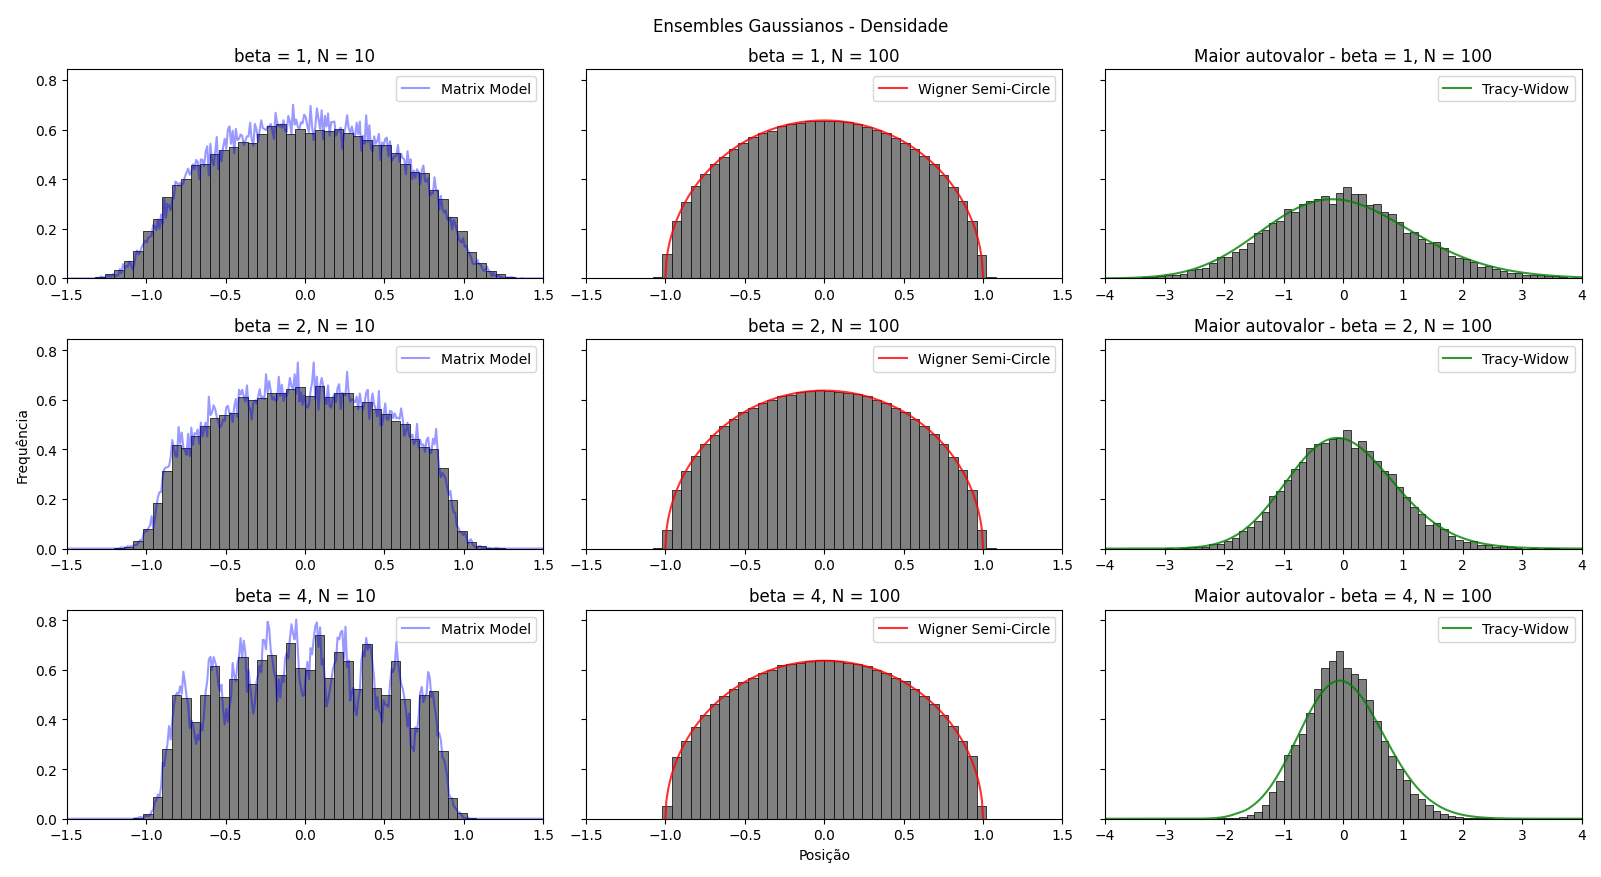
\includegraphics[width=0.9\textwidth]{Assets/validationGaussianTracy.png}
	\caption{Densidade para ensembles gaussianos, \ref{Equation: Parametros Gaussian}. Tomou-se $\Delta t = 0.3$ e $nsteps = 5\cdot10^6$ passos, registrando a cada $1000$ iterações a partir de $nsteps/5$. À esquerda da figura, em azul, a densidade da amostragem de $4\cdot10^3$ matrizes do ensemble. No centro, o Semi-Círculo de Wigner, medida de equilíbrio. Na direita, apresenta-se a densidade de $\lambda_{max}$ normalizado e sua mediada esperada.}
	\label{Figura: Gaussian}
\end{figure}

Indo além dos modelos gaussianos podemos retomar as descrições dos potenciais mônico e quártico. Respectivamente, estes modelos equivalem a tomar na simulação os parâmetros $d = 1, \ \  n = 2, \ \ \beta_N = \beta N^2$ para $\beta = 2$ com
\begin{equation}
	\V(x)= t |x|^{2m}, \ \ W(x) = g(x) = \log{|x|}.
	\label{Equation: Parametros Monico}
\end{equation}
e $d = 1, \ \  n = 2, \ \ \beta_N = \beta N^2$ para $\beta = 2$ com
\begin{equation}
	\V(x)=\frac{|x|^4}{4} + t \frac{|x|^2}{2}, \ \ W(x) = g(x) = \log{|x|}.
	\label{Equation: Parametros Quartico}
\end{equation}
O caso mônico se reduz ao gaussiano se $m=1$. Os resultados para ambos os potenciais estão explicitados na Figura \ref{Figura: Quartic Monic} para alguns parâmetros interessantes de $t$ e $m$.
\begin{figure}[ht!]
	\centering
	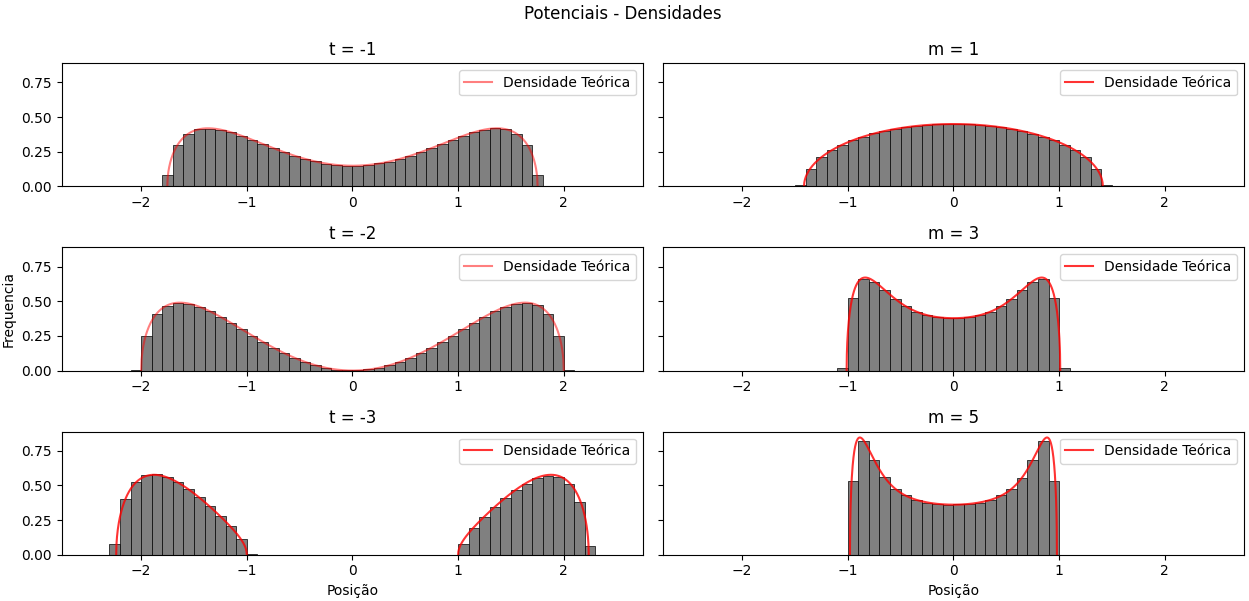
\includegraphics[width=0.8\textwidth]{Assets/validationQuarticMonic-alt.png}
	\caption{Potencial Quártico \ref{Equation: Parametros Quartico} e Mônico \ref{Equation: Parametros Monico}, respectivamente à esquerda e direita. Tomou-se $\Delta t = 0.1$, $N=100$, e $nsteps = 5\cdot10^6$ passos. Registra-se a cada $1000$ iterações a partir de $nsteps/5$. No Quártico, simula-se $t=-1,-2,-3$. No Mônico fixa-se $t=1$ e simula-se $m=1,3,5$.}
	\label{Figura: Quartic Monic}
\end{figure}

É fácil ver para os casos \ref{Equation: Parametros Gaussian}, \ref{Equation: Parametros Monico}, \ref{Equation: Parametros Quartico} que as medidas explícita pela teoria são concordantes, como esperado, com a medida experimental obtida nas simulações. Contudo, isso é bem explorado e pode ser observado, com exceção do Mônico, em \cite{Chafa2018}.

 Em uma situação menos explorada, considere a seguinte configuração de potencial e autovalores complexos ($\R^d = \R^2$) e a representação das medidas simuladas para alguns valores de interesse de $t, a$ na Figura \ref{Figura: Complex},
\begin{equation}
	d = 2; \  n = 2; \  \V(z)=|z|^{2a} - \Re{t z^a};  \ W(x) = g(x) = \log{|x|};  \ \beta_N = \beta N^2;  \ \beta = 2.
	\label{Equation: Complex}
\end{equation}

\begin{figure}[h]
	\centering
	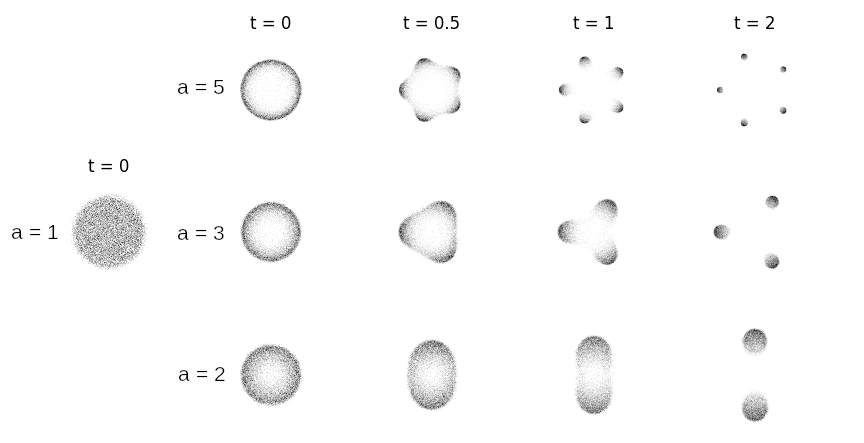
\includegraphics[width=0.8\textwidth]{Assets/complexPotential.png}
	\caption{Medidas referentes à configuração \ref{Equation: Complex}. Tomou-se $\Delta t = 0.5$ e $nsteps = 2\cdot10^6$ passos, registrando a cada $500$ iterações a partir de $nsteps/5$.}
	\label{Figura: Complex}
\end{figure}

É previsto para esse modelo uma transição de regime, uma separação da medida de equilíbrio, para $t_c \approx \sqrt{\frac{1}{a}}$ \cite{balogh2016orthogonal}. A simulação replicar o comportamento esperado é um bom indicador de que é possível estudar a medida de tal ensemble numericamente, que pode ser explorado posteriormente. Outro fator que corrobora o bom comportamento do modelo é a medida uniforme quando $a=1$, também prevista pela teoria. 

%Outro potencial explorado pela literatura é descrito por
%\begin{equation}
%	d = 2; \  n = 2; \  \V(z)=\frac{1}{t_1}\left(|z|^{2} - 2\Re{\frac{z^{3}}{3} + t_0 z}\right);  \ W(x) = g(x) = \log{|x|};  \ \beta_N = \beta N^2;  \ \beta = 2.
%	\label{Equation: ComplexDiagram}
%\end{equation}
%para o qual podemos representar uma seção de relevância do diagrama de fase para $(t_0, t_1)$ com ofeito na \ref{Figura: ComplexDiagram}

%\begin{figure}[h]
%	\centering
%	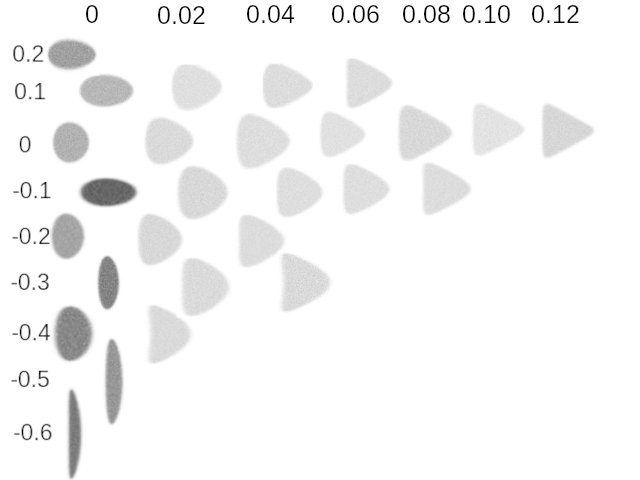
\includegraphics[width=0.6\textwidth]{Assets/allshapes.png}
%	\caption{Medidas referentes à configuração \ref{Equation: ComplexDiagram}. Tomou-se $\Delta t = 0.5$ e $nsteps = 2\cdot10^6$ passos, registrando a cada $500$ iterações a partir de $nsteps/5$. horizontalmnete varia-se $t_1$, verticalmente $t_0$.}
%	\label{Figura: ComplexDiagram}
%\end{figure}

%Os resultados são holísticos mas parecem concordar com as previsões da literatura, como em \cite{Guilherme}.
Notamos que os modelos gaussianos são os únicos em RMT com invariância por rotação e independência das entradas simultaneamente. Gerar matrizes de outros modelos invariantes dependeria de gerar entradas correlacionadas ja que, se tratando de ensembles invariantes, ou seja, de medida igual para quaisquer $M, M'$ tais que $\matriz{M} = \matriz{U} \matriz{M'} \matriz{U}^{-1}$, podemos simular $\matriz{U}$ autovetores uniformemente do espaço correspondente. Isso pois sabemos do teorema espectral que, para as matrizes tomadas, vale a decomposição $\matriz{M} = \matriz{U} \matriz{D} \matriz{U}^{-1}$. Para reconstruir uma elemento do ensemble de interesse nos resta replicar a medida de autovalores, $\matriz{D}$. Isso, de forma interessante, pode ser feito pela simulação descrita de Gases de Coulomb, que replica a medida dos ensemble.

\subsection{Conclusão}

Descrevemos os fundamentos da Teoria de Matrizes Aleatórias e, com essas ideias, explicitamos os modelos gaussiano para $\beta = 1,2,4$, importantes em RMT pela sua característica única de pertencer à ambas categorias de ensembles, invariantes e independentes. Usando desse exemplo podemos entender os principais resultados sobre medidas dos ensembles invariantes e sobre a medida de autovalores destas matrizes. 

Introduzimos a ideia de um Gás de Coulomb e como esta noção pode ser relacionada com os ensembles de matrizes aleatórias. Usando da ideia de partículas para pensar na dinâmica dos autovalores intuímos as ideias de minimização da energia livre para identificar o equilíbrio. Com isso, mostramos os principais resultados que possibilitam o cálculo explicito da medida de autovalores para o caso gaussiano e mais dois ensembles que usaremos como exemplo nas simulações que seguem. Com a analogia, percebemos que muitas vezes métodos numéricos são necessários para a solução das equações de movimento de descrevem a dinâmica das partículas descritas. Discutimos os principais métodos e principalmente as características do algoritmo implementado, justificando seu uso e propondo sua forma final apresentada também neste trabalho.

Por fim, apresentamos os resultados. Simulações de medidas para os ensembles já descritos anteriormente, todos com autovalores reais, e um último ensemble com autovalores complexos, menos descrito. Para os efeitos deste trabalho, foi encontrada boa concordância das medidas simuladas com a descrição teórica atual e com os modelos de matriz testados. Principalmente para o ensemble de autovalores complexos, este resultado é de interesse visto que apresenta uma forma alternativa de simulação e, também, de análise numérica destes modelos para diversos ensembles explorados em literatura recente.

Finalmente, entendemos os resultados deste estudo como uma descrição e validação de métodos conhecidos de simulação e estudo de matrizes aleatórias, ainda que atuais. Contudo, vê-se extensões da utilização do método para estudo numérico de importantes resultados com pouca descrição teórica.

%%-----
%% Referências bibliográficas
%%-----
\addcontentsline{toc}{chapter}{\bibname}
\bibliographystyle{abntex2-num}
\bibliography{bibliografia}

%%-----
%% Fim do documento
%%-----

%\appendix
%\chapter{Implementação Algoritmo}

%\inputminted[
%frame=lines,
%framesep=2mm,
%baselinestretch=1.2,
%bgcolor=white,
%fontsize=\footnotesize,
%linenos
%]{FORTRAN}{Assets/HKMC.f}

\end{document}